% begin module tangents-reminder
\begin{frame}
\frametitle{Tangents}
\begin{center}
\psset{xunit=0.8cm, yunit=0.8cm}
\begin{pspicture}(-2.7, -0.7)(2.7,6.4)
\tiny
\fcLabelXOne
\fcLabelYOne
\rput[l](0.2, 3.5){$y=x^2$}
\psaxes[ticks=none, labels=none]{<->}(0,0)(-1,-0.5)(2.5,4.5)
%Function formula: (x)^{2}
\psplot[linecolor=red, plotpoints=1000]{-1}{2.5}{x 2 exp }
\psline[linecolor=blue](0.25, -0.5)(2.5,4)
\fcFullDot{1}{1}
\rput[lt](1.1, 0.9){$P=(1,1)$}
\end{pspicture}
%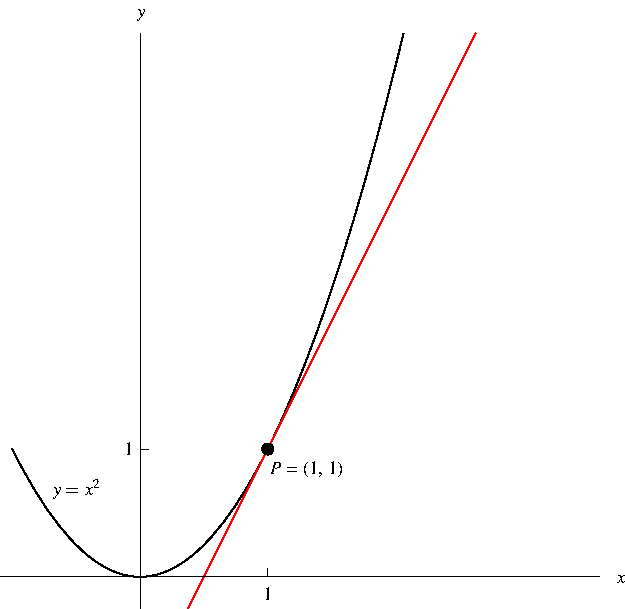
\includegraphics[height=5cm]{derivatives/pictures/02-01-secanta.pdf}%
\end{center}
\begin{itemize}
\item<2->  Recall that in preceding lectures we tried to find the tangent line to the curve $y = x^2$ at the point $P = (1,1)$.
\item<3->  This problem motivated us to study limits.
\end{itemize}
\end{frame}


% end module tangents-reminder
